%%%%%%%%%%%%%%%%%%%%%%%%%%%%%%%%%%%%%%%%%%%%%%%%%%%%%%%%%%%%%%%%%%%%%
%
% 1.pdflatex main.tex 2.bibtex main.aux 3. pdflatex  main.tex 4. pdflatex  main.tex
%%%%%%%%%%%%%%%%%%%%%%%%%%%%%%%%%%%%%%%%%%%%%%%%%%%%%%%%%%%%%%%%%%%%%%

\documentclass[11pt]{article}
\usepackage{tabularx}
\newcolumntype{b}{X}
\newcolumntype{s}{>{\hsize=.5\hsize}X}
%\usepackage[spanish]{babel}
\usepackage[english]{babel}
%\usepackage[osf]{mathpazo}
%\usepackage{bookman}
\usepackage{palatino}
\usepackage[utf8]{inputenc}
\usepackage[utf8]{luainputenc}
%\usepackage{floatrow}

%\usepackage[T1]{fontenc}
%\usepackage{pgffor}
%\usepackage{lipsum}
%\usepackage[OT1]{fontenc}
\usepackage[a4paper]{geometry}
\usepackage[myheadings]{fullpage}
\usepackage{fancyhdr}
\usepackage{lastpage}
\usepackage{amsfonts, amsmath, amsthm, amssymb}
\theoremstyle{definition}
\newtheorem{definition}{Definition}[section]
 
\theoremstyle{remark}
\newtheorem*{remark}{Remark}
\DeclareMathOperator*{\argmax}{arg\,max}
\DeclareMathOperator*{\argmin}{arg\,min}
\usepackage{graphicx, wrapfig, subcaption, setspace, booktabs}
\usepackage[T1]{fontenc}
\usepackage[font=small, labelfont=bf]{caption}
\usepackage{fourier}
\usepackage{float}
%\usepackage[protrusion=true, expansion=true]{microtype}
%\usepackage[margin=1in]{geometry}
\usepackage{microtype}
\usepackage{sectsty}
\usepackage{url, lipsum}
\usepackage{listings}
\usepackage{xcolor}
\newcounter{countCode}
\newcommand{\HRule}[1]{\rule{\linewidth}{#1}}
\onehalfspacing
\setcounter{tocdepth}{5}
\setcounter{secnumdepth}{5}
\lstnewenvironment{code} [1][caption=Ponme caption, label=default]{%
\renewcommand*{\lstlistingname}{Python} 
  \setcounter{lstlisting}{\value{countCode}} 
  \lstset{ %
  language=python,
  basicstyle=\ttfamily\footnotesize,       % the size of the fonts that are used for the code
  numbers=left,                   % where to put the line-numbers
  numberstyle=\sc,      % the size of the fonts that are used for the line-numbers
  stepnumber=1,                   % the step between two line-numbers. 
  numbersep=5pt,                 % how far the line-numbers are from the code
  numberstyle=\color{red!50!blue},
    backgroundcolor=\color{lightgray!20},
  rulecolor=\color{blue},
  keywordstyle=\color{red}\bfseries,
  showspaces=false,               % show spaces adding particular underscores
  showstringspaces=false,         % underline spaces within strings
  showtabs=false,                 % show tabs within strings adding particular underscores
  frame=single,                   % adds a frame around the code
  framexleftmargin=0mm,
  numberblanklines=false,
  xleftmargin=5pt,
  breaklines=true,
  breakatwhitespace=true,
  breakautoindent=true,
  captionpos=t,
  texcl=true,
  tabsize=2,                      % sets default tabsize to 3 spaces
  extendedchars=true,
  inputencoding=utf8, 
  escapechar=\%,
  morekeywords={print, println, size, background, strokeWeight, fill, line, rect, ellipse, triangle, arc, save, PI, HALF_PI, QUARTER_PI, TAU, TWO_PI, width, height,},
  emph=[1]{print,println,}, emphstyle=[1]{\color{blue}}, % Mis palabras clave.
  emph=[2]{width,height,}, emphstyle=[2]{\bf\color{violet}}, % Mis palabras clave.
  emph=[3]{PI, HALF_PI, QUARTER_PI, TAU, TWO_PI}, emphstyle=[3]\color{orange!50!violet}, % Mis palabras clave.
  emph=[4]{line, rect, ellipse, triangle, arc,}, emphstyle=[4]\color{green!70!black}, % Mis palabras clave.
  %emph=[5]{size, background, strokeWeight, fill,}, emphstyle=[5]{\tt \color{red!30!blue}}, % Mis palabras clave.
  %emph={[2]sqrt,baset}, emphstyle={[2]\color{blue}}, % f(sqrt(2)), sqrt a nivel 2 se pondrá azul
#1}}{\addtocounter{countCode}{1}}
%-------------------------------------------------------------------------------
% HEADER & FOOTER
%-------------------------------------------------------------------------------
\pagestyle{fancy}
\fancyhf{}
\setlength\headheight{12pt}
\fancyhead[L]{Seven years of \emph{Proyecto Vallecas}}
\fancyhead[R]{Gómez-Ramírez et al. Fundaci\'on CIEN}
\fancyfoot[R]{\small{page} \thepage\ \small{of} \pageref{LastPage}}
%-------------------------------------------------------------------------------
% TITLE PAGE
%-------------------------------------------------------------------------------

\begin{document}
%IDENTIFICACIÓN DE FACTORES DE RIESGO EN DETERIORO COGNITIVO LEVE CON APRENDIZAJE AUTOMÁTICO: HACIA UNA AYUDA AL DIAGNÓSTICO MULTIFACTORIAL Y  AUTOINFORMADA

\title{ \normalsize \textsc{\emph{Proyecto Vallecas} Seven years longitudinal study in healthy aging}
    \\ [2.0cm]
    \HRule{0.5pt} \\
    \LARGE \textbf{\uppercase{Exploratory Data Analysis in \emph{Proyecto Vallecas}: a seven years longitudinal study in brain healthy aging}}
    \HRule{2pt} \\ [0.5cm]
    \normalsize \today \vspace*{5\baselineskip}}

\date{ }
\author{
    Jaime G\'omez-Ram\'irez, Marina \'Avila Villanueva, Bel\'en Frades Payo, Teodoro del Ser Quijano,\\ Meritxell Valent\'i Soler, María Ascensi\'on Zea Sevilla and Miguel \'Angel Fern\'andez-Bl\'azquez   \\  \\
    \textbf{\large{Fundaci\'on Reina Sof\'ia}} \\
    Centre for Research in Neurodegenarative Diseases
    \\ \emph{Valderrebollo, 5, 28031 Madrid}
 }

\maketitle
\begin{center}

\includegraphics[width = 60mm]{figures/logo_mciu.png}
\end{center}
\newpage
\tableofcontents
\newpage

%-------------------------------------------------------------------------------
% Section title formatting
\sectionfont{\scshape}
%-------------------------------------------------------------------------------

%-------------------------------------------------------------------------------
% BODY

%CODE
%tensorflow/production/descriptive_stats.py
%-------------------------------------------------------------------------------

\section*{Abstract}
Alzheimer's Disease (AD) is a complex, multifactorial and comorbid condition. The asymptomatic behavior in early stages of the disease is a paramount obstacle to formulate a preclinical and predictive model of AD. Not surprisingly, the AD drug approval rate is one of the lowest in the industry, an exiguous $0.4\%$. The identification of risk factors, preferably obtained by the subject herself, is sorely needed given that the incidence of Alzheimer’s disease grows exponentially with age. 

During the last 7 years, researchers at \emph{Proyecto Vallecas} have collected information about the project's volunteers, aged 70 or more. The \emph{Proyecto Vallecas} dataset includes information about a wide range of factors including genetic, demographic, socioeconomic, cognitive performance, subjective memory complains, neuropsychiatric disorders, cardiovascular, sleep, diet, physical exercise and self assessed quality of life. The subjects in each visit were diagnosed as healthy, mild cognitive impairment (MCI) or dementia. 
%'CognitivePerformance', 'Diagnoses', 'Neuropsychiatric', 'QualityOfLife', 'Genetics_s', 'SCD', 'Demographics', 'Cardiovascular_s', 'PhysicalExercise_s', 'Sleep_s', 'Anthropometric_s', 'Diet_s', 'SocialEngagement_s', 'TraumaticBrainInjury_s', 'Demographics_s', 'EngagementExternalWorld_s'

In this study we perform Exploratory Data Analysis to summarize the main characteristics of this unique longitudinal dataset. The objective is to characterize the evolution of the collected features over time and most importantly, how their dynamics are related to cognitive decline. 
We identify time series characteristics with predictive power about cognitive decline. We show that the longitudinal dataset of \emph{Proyecto Vallecas}, if conveniently exploited, holds promise to identifying either factors promoting healthy aging and risk factors related to cognitive decline. 
 
\section{Introduction}
\label{se:int}
The Vallecas Project for early detection of AD is the most ambitious population-based study for healthy aging in Spain. The project is carried out at the Queen Sofia Foundation Alzheimer Center by a multidisciplinary team of researchers from the CIEN Foundation. The main objective of the Vallecas Project is to elucidate, through tracking of progression of the cohort, the best combination of features, clinical and others that are informative about developing cognitive impairment in the future. 
%Thus, it intends to identify a set of \emph{markers} to eventually determine the potential risk that an individual has to develop the disease in the future. 

The dataset at its inception in the first year contained 1,213 subjects who were described using a large range of features most of them collected yearly. 
It is worth noting that the data set contains two types of observations: variables and time series. The former refer to variables that are measured only once, typically in the first year's visit (e.g. APOE genotyping or educational attainment) and the later are variables with a time index attached (time series) measured at every subject's visit (e.g. results of cognitive performance test, subjective memory complains).
Importantly, the dimensionality of the dataset grows every year (new measurements of features are added) as it does the number of samples as the subjects keep coming for their yearly visits, however the number of examples collected per year decreases (some volunteers drop the study). Table \ref{fig:tableclustervallecas} shows the features types that are collected in the study.

\begin{table}
\begin{tabular}{ |p{4cm}|p{4cm}|p{4cm}| }
\hline
\hline
MRI & Genetics(APOE) & Demographics  \\
\hline
Anthropometric & Sleep & Quality of life \\
\hline
Cognitive performance & Subjective memory complains & Diet \\
\hline
Physical exercise & Diagnoses & Neuropsychiatric \\
\hline
Traumatic brain injury & Engagement external world &  \\
\hline

\hline
\end{tabular}
\caption{\label{tab:tableclustervallecas} Category of features included in the dataset. Each item in the table refers to a set of variables collected. Note that some features are collected only during the first year (basal) for example Genetics(APOE) or Demographics e.g. level of education, but for the most part, features are assessed for every year's visit by the team of neuropsychologists and neurologists.}
\end{table}

The structure of the document is as follows. 
Section \cite{se:int} provides a comprehensive description of the information collected, the description relies upon visual charts and we also study the distribution of some key features collected in \emph{Proyecto Vallecas} dataset.
Section \ref{se:met} shows statistical tests and the correlation analysis paying special attention to the evolution of the longitudinal variables and their underlying relationship with cognitive performance. 
Section \ref{se:met} describes the features that are most strongly related to cognitive decline for both static (measured once) and dynamic variables (measured every year). We extract features from the longitudinal features to build a classifier based on relevant features extracted from time series \cite{christ2018time}. We conclude with the discussion of the results and future works in Section \ref{se:con} connecting our findings with previous populational studies.  

% YS give full description of features
% Description of the dataset table with all features
% draw time line of the prj

%Sleep
%Diet APOE
%'Cardiovascular_s', 'PhysicalExercise_s', 'Sleep_s', 'Anthropometric_s', 'Diet_s', 'SocialEngagement_s', 'TraumaticBrainInjury_s', 'Demographics_s', 'EngagementExternalWorld_s'

\subsection{Exploratory Data Analysis static variables}
%Static as the correlate with conversion
In this section we perform Exploratory Data Analysis (EDA). The objective of EDA is to build graphical representations that help us make sense of the data. EDA gives us a bird's eye of the dataset to help us identifying patterns and trends and most importantly, assist us in framing the type of questions we want to ask.
EDA relies upon a careful pre-processing of the dataset. We perform EDA in a succession of steps, we will start with data understanding where we will plot charts containing basic information of the dataset like the age distribution and other demographics of the participants. 
We will also study the distribution of the most significant features of all type of features depicted in \ref{tab:tableclustervallecas}. Furthermore we plot the distribution of cognitive decline conditional to other features. This will set the stage for the correlation analysis described in Section \ref{se:res} for both static (one observation) and dynamic variables (time series). 

%%EDA paper1: Here we perform Exploratory Data Analysis (EDA). EDA is the first step in the data analysis process and is performed once the pre processing steps have finished. 
The total number of visits collected in the so far 7 years project is 4444. Figure \ref{fig:pv5years}depicts the number of volunteers for the seven years life of the project.

\begin{figure}[H]
        \centering
        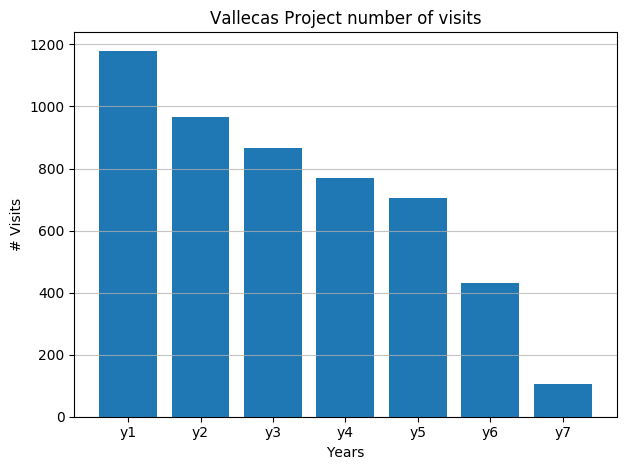
\includegraphics[keepaspectratio, width=0.5\linewidth]{figures/Fig_visits}
        \caption{Number of volunteers across seven years of \emph{Proyecto Vallecas}. As expected, the number of subjects decreases across time. The number of subjects in the year 1 was 1213 of which 33 were removed because were diagnosed with MCI or AD resulting in 1180 subjects recruited to participate in the study in year 1. 965 of the initial 1180 came for a second visit ($18\%$ drop rate), 865 in year 3 ($27\%$ drop rate from year 1), 770 in year 4 ($35\%$ drop rate from year 1), 704 in year 5 ($40\%$ drop rate from year 1), 431 in year 6(($63\%$ drop rate from year 1)) and 107 in year 7 which at this moment still ongoing ($91\%$ drop rate from year 1). The total number of visits in five years amounts to 5022.} \label{fig:pv5years}
\end{figure}


% features_dict['Anthropometric_s'] == ['lat_manual', 'pabd', 'peso', 'talla', 'audi', 'visu', 'imc']
% Plot 'pabd', 'peso', 'talla', 'audi'
Figure \ref{fig:anthro} shows the histogram for anthropometric variables bmi, abdominal perimeter, weight and height, measured at year 1.
\begin{figure}[H]
        \centering
        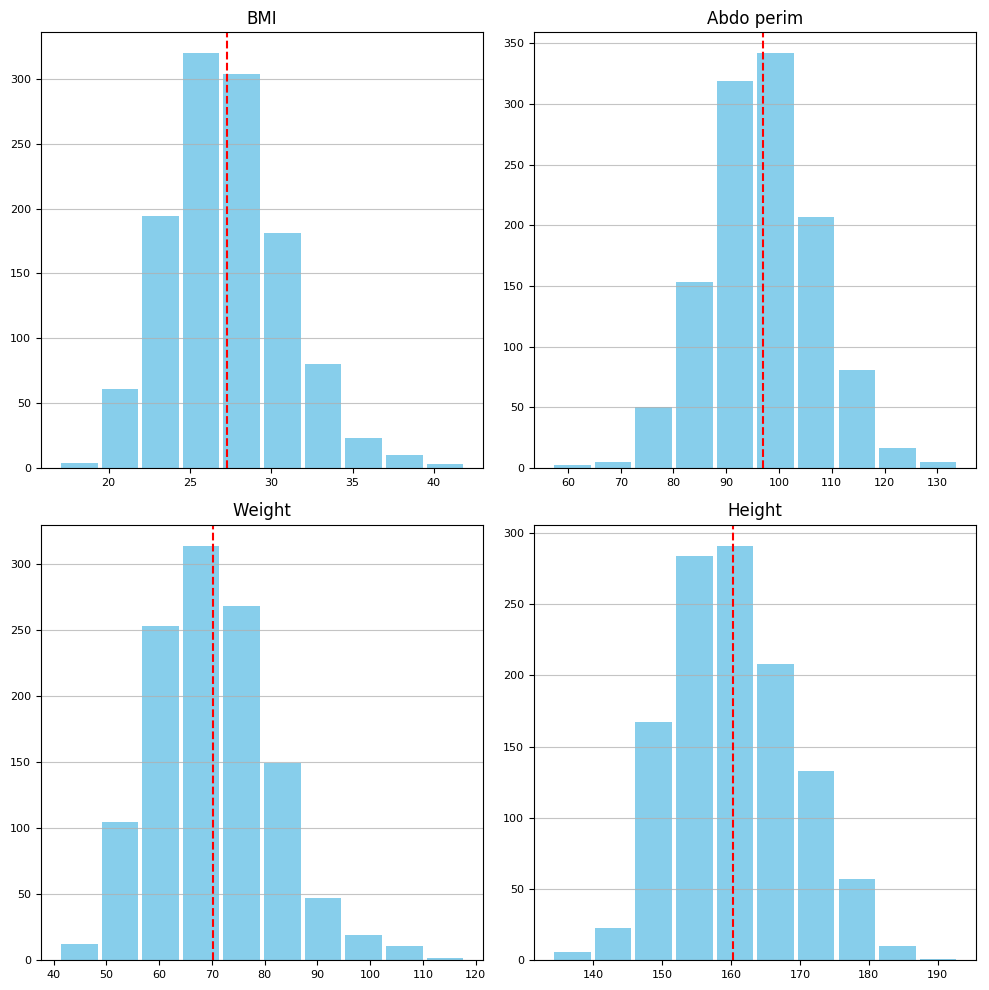
\includegraphics[keepaspectratio, width=0.5\linewidth]{figures/Fig_anthro}
        \caption{Histogram of anthropometric variables measured in year 1 of \emph{Proyecto Vallecas} dataset. Clockwise, Body Mass Index (min=16.95, max=41.93), abdominal perimeter (min=57cm, max=134cm), weight (min=41kg, max=118kg) and height(min=134cm, max=193cm)} 
        \label{fig:anthro}
\end{figure}

Figure \ref{fig:sexlat} shows the histogram for sex and hand laterality.
\begin{figure}[H]
        \centering
        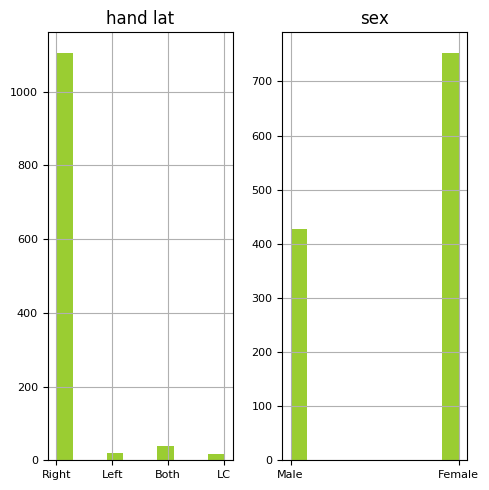
\includegraphics[keepaspectratio, width=0.5\linewidth]{figures/Fig_sexlat}
        \caption{Histogram of sex and hand laterality in year 1. There is majority of females, 753 versus 427. The right handed are 1106, left 19, ambidextrous 39 and 16 were forced right abut born left.} 
        \label{fig:anthro}
\end{figure}

% features_dict['Demographics_s'] == ['edad', 'edad_visita7']
Figures \ref{fig:ages} and \ref{fig:ages} show the histogram for demographic variables. Figure \ref{fig:ages} depicts the age of the participants at the inception of the project and the age of the participants that came to the seventh visit.

\begin{figure}[H]
        \centering
        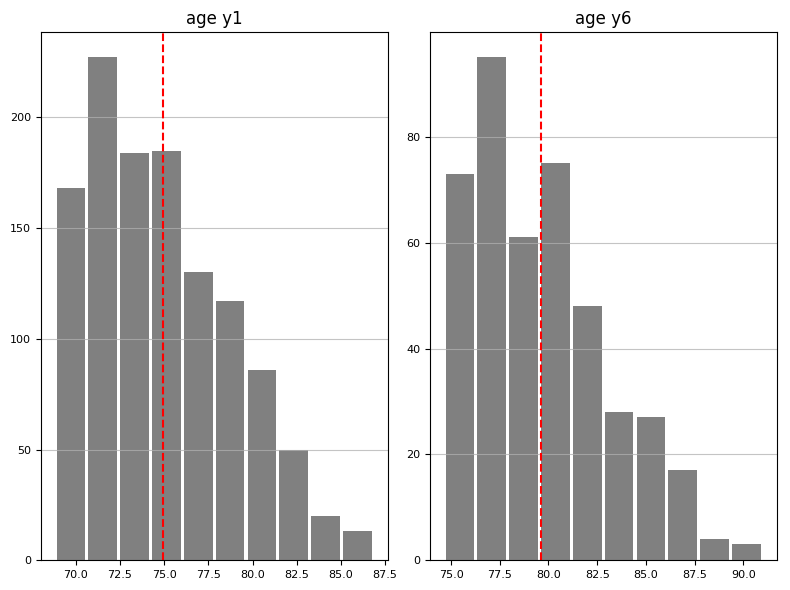
\includegraphics[keepaspectratio, width=0.5\linewidth]{figures/Fig_ages}
        \caption{Histogram of the age of the participants in the first and last year of the \emph{Proyecto Vallecas} dataset. The youngest and the oldest participant in year 1 were 69 and 86 years old. In year 7 the minimum and maximum ages are 76 and 89.} 
        \label{fig:anthro}
\end{figure}

%['renta', 'nivelrenta', 'educrenta', 'municipio', 'barrio', 'distrito', 'sexo', 'nivel_educativo', 'anos_escolaridad', 'familial_ad', 'sdestciv', 'sdhijos', 'numhij', 'sdvive', 'sdocupac', 'sdresid', 'sdtrabaja', 'sdeconom', 'sdatrb']

Figure \ref{fig:apoe} the APOE Genotyping test classifying the subjects in three groups depending on whether they have no copy of the APO$\epsilon4$ allele one copy ApoE4 heterozygotes or two copies APO$\epsilon4$ APO$\epsilon4$ \cite{farrer1997effects}. The APO$\epsilon4$ variant is the largest known genetic risk factor for late-onset sporadic Alzheimer's disease (AD), however the correlation with risk changes with ethnicity, for example Nigerian blacks have the highest observed frequency of the APO$\epsilon4$ allele in world populations, but AD is apparently less frequent than in other populations \cite{sepehrnia1989genetic}.
Estimated worldwide human allele frequencies of ApoE is $13.7\%$ and $36.7\%$ in AD patients. On the other hand, $40–65\%$ of AD patients have at least one copy of the APO$\epsilon4$ allele.

In our population, $82\%$ were APO$\epsilon4$ negative, $17\%$ APO$\epsilon4$ heterozygotes and $1\%$ APO$\epsilon4$ homozygotes. 
%DO p(AD|+ in apoe)

\begin{figure}[H]
        \centering
        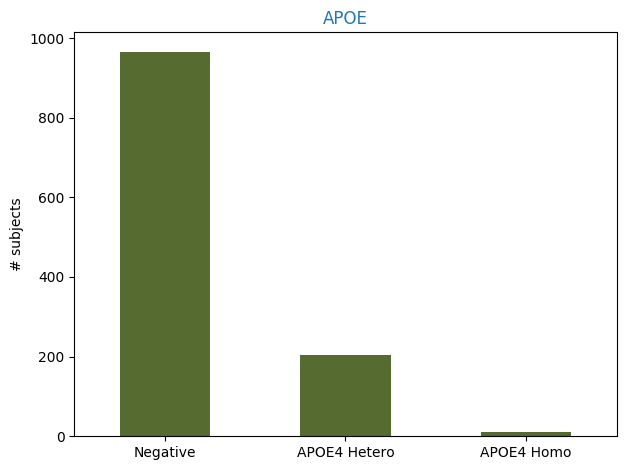
\includegraphics[keepaspectratio, width=0.5\linewidth]{figures/Fig_apoe}
        \caption{APOE Genotyping testing in \emph{Proyecto Vallecas} dataset. $17\%$ of subjects carry at least one copy of the $\epsilon4$, slightly higher than the worldwide in Caucasian population described ($13.7\%$ ) as estimated in \cite{farrer1997effects}} 
        \label{fig:demo}
\end{figure}

Figure \ref{fig:ages} depicts the rest of demographic variables including: educational attainment,  number of sons, years of work as an employee, self-assessed economic status,marital status and the  number of people living at home.
\begin{figure}[H]
        \centering
        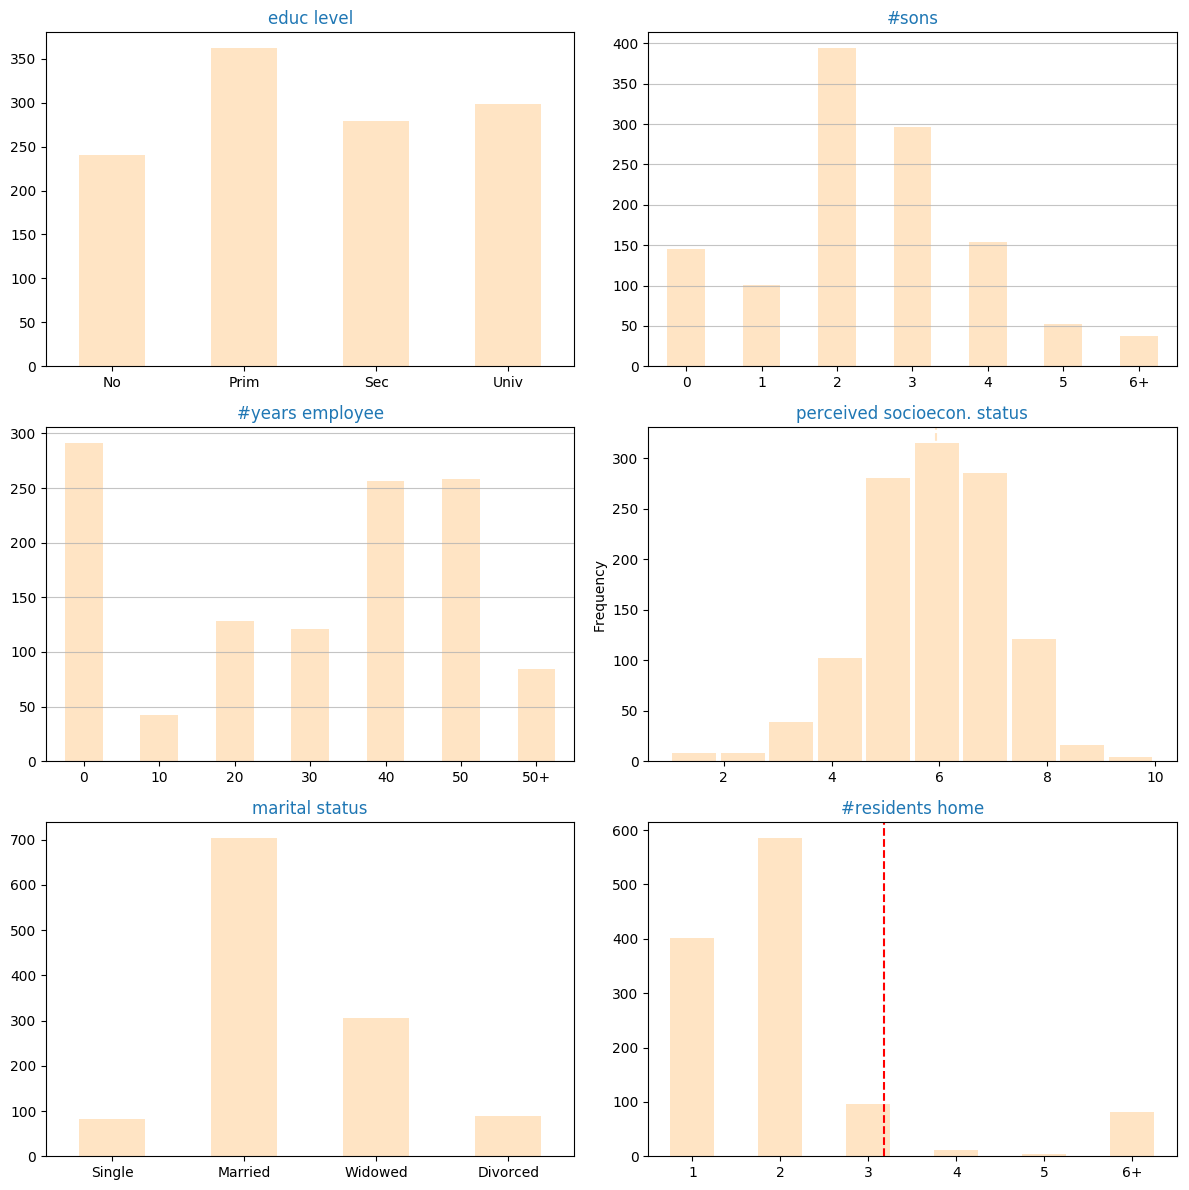
\includegraphics[keepaspectratio, width=0.5\linewidth]{figures/Fig_demo}
        \caption{Histogram of demographic variables in the \emph{Proyecto Vallecas} dataset in the first year. Clockwise, educational attainment (No formal education, primary school, secondary school and university),  number of sons, number of years of work as an employee, self-assessed economic status (1 the lowest, 10 the highest, marital status (single, married, widows and divorced) and the  number of people living at home.} 
        \label{fig:demo}
\end{figure}

Figure \ref{fig:sleep} depicts features related to sleep patterns of the subjects. Daily naps are less common that what it could be expected from a Spaniard population aged 70 or more. $37\%$ of subjects do not take any nap at all, $24\%$ of subjects sleep daily between 15 and 30 minutes and the $17$ report to take naps of at least one hour a day. The majority of subjects report remembering their dreams $67.7\%$ versus $32\%$ that do not. The majority of subjects report to snore during sleep $60\%$. 

\begin{figure}[H]
        \centering
        \includegraphics[keepaspectratio, width=\linewidth]{figures/Fig_sleep}
        \caption{Histogram of sleep variables in the \emph{Proyecto Vallecas} dataset in the first year. From left to right and up to the bottom, number of hours of sleep during the day ($\mu=0.45, \sigma=1$), tingling during sleep (0 No, 1 Yes, 9 Dk/Da), movements during sleep (0 No, 1 Yes, 9 Dk/Da), number of hours of night sleep ($\mu=6.8, \sigma=1.3$), deep sleep (1 Light, 2 Moderate, 3 Deep), remember dreams (0 No, 1 Yes, 9 Dk/Da), snoring (0 No, 1 Yes, 2 snore and difficult breathing 9 Dk/Da), noises during sleep (0 No, 1 Yes, 9 Dk/Da), sufficient sleep (0 No, 1 Yes, 9 Dk/Da).} 
        \label{fig:demo}
\end{figure}

Figure \ref{fig:incomeresidency} shows the home residency and the income distribution of \emph{Proyecto Vallecas} subjects as estimated based on their home residency. A more in detail representation of the home residency is shown in figure \ref{fig:resid_detail}

\begin{figure}[H]
        \centering
        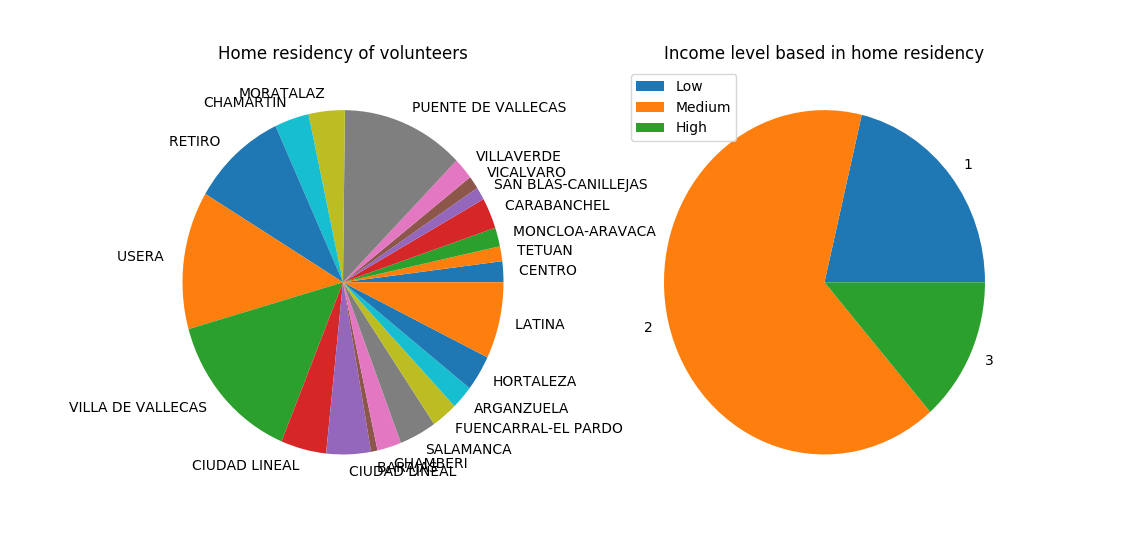
\includegraphics[keepaspectratio, width=\linewidth]{figures/incomeresidency}
        \caption{On the left, distribution of home residency by districts of \emph{Proyecto Vallecas} volunteers in year 1. All districts of the city of Madrid are represented. Note that there are 156 subjects of a total of 1180 that are not residents in the city of Madrid and are not included here. On the right, we plot the income distribution as estimated based on the home residency, 251 subjects live in low income areas, 769 in medium income areas and 160 in high income neighborhoods of Madrid.
        } \label{fig:incomeresidency}
\end{figure}

\begin{figure}[]
        \centering
        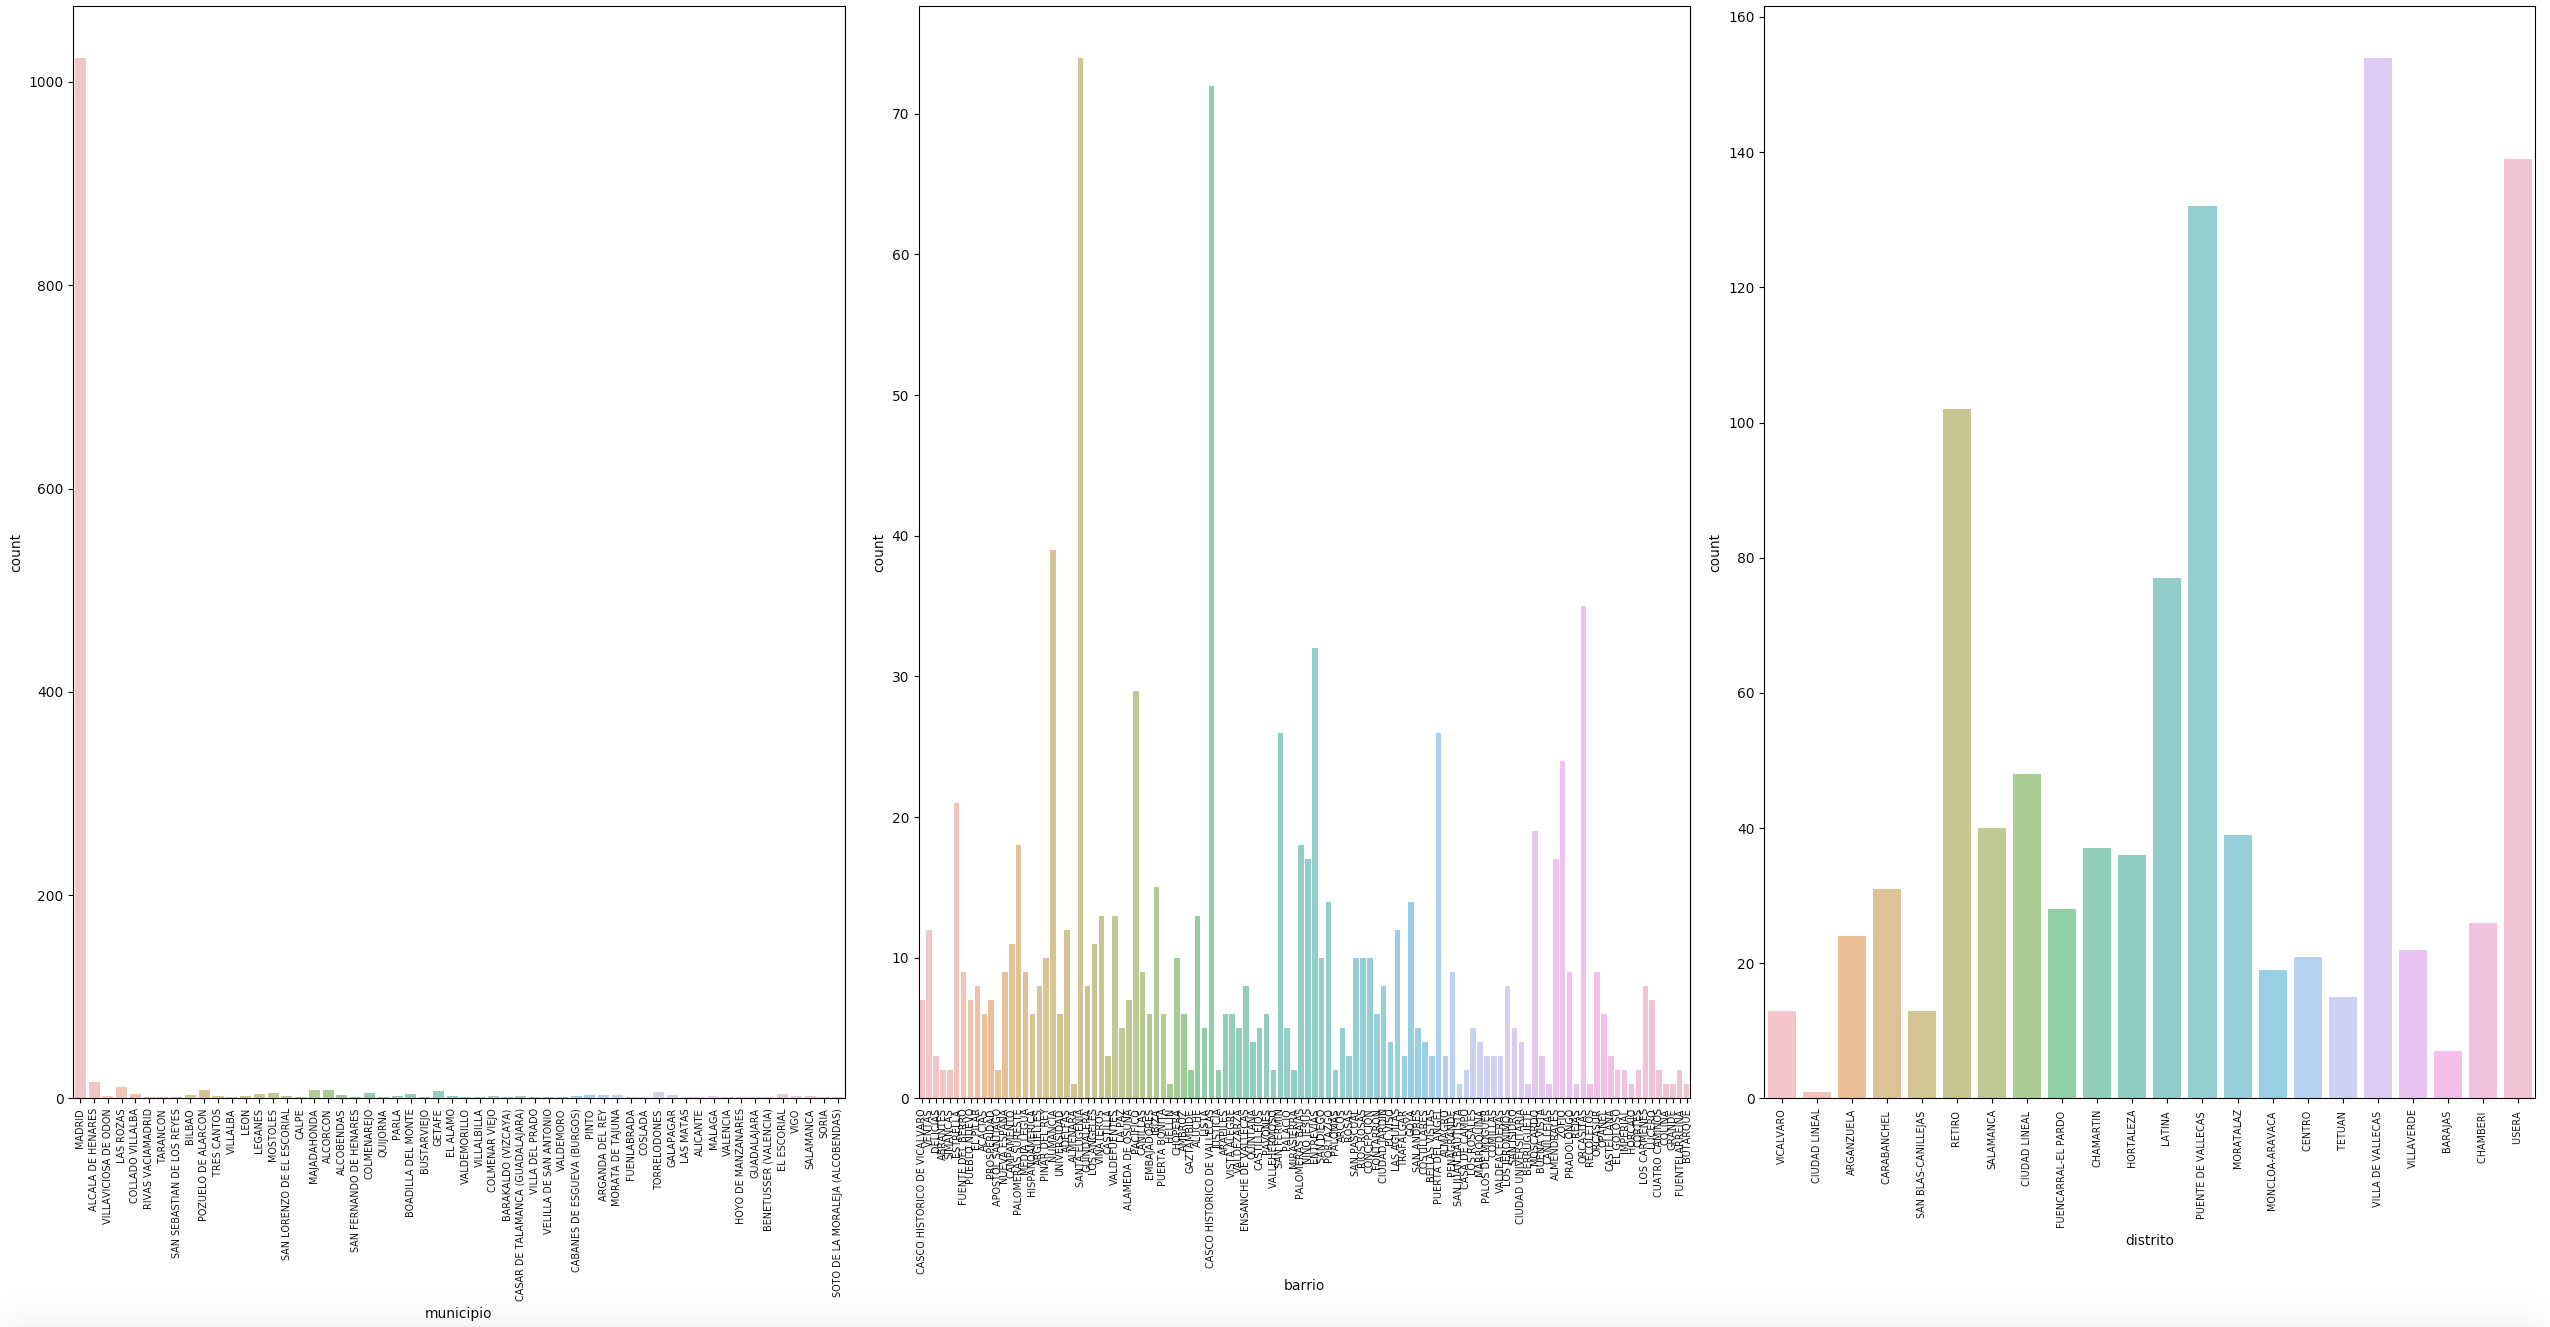
\includegraphics[height=\textheight, width=\textwidth]{figures/resid_detail}
        \caption{On the left, city of residency of subjects, the large majority lives in Madrid. Middle figure neighborhood and right figure borough of residence in the city of Madrid. 
        } \label{fig:incomeresidency}
\end{figure}

% Food
Figure \ref{fig:food} depicts the type of food consumption reported by the subjects. $84\%$ of subjects report to consume olive oil 6/7 days a week, $74\%$ bread, $44\%$ vegetables and $29\%$ report consuming sweets 6/7 days a week.

\begin{figure}[H]
        \centering
        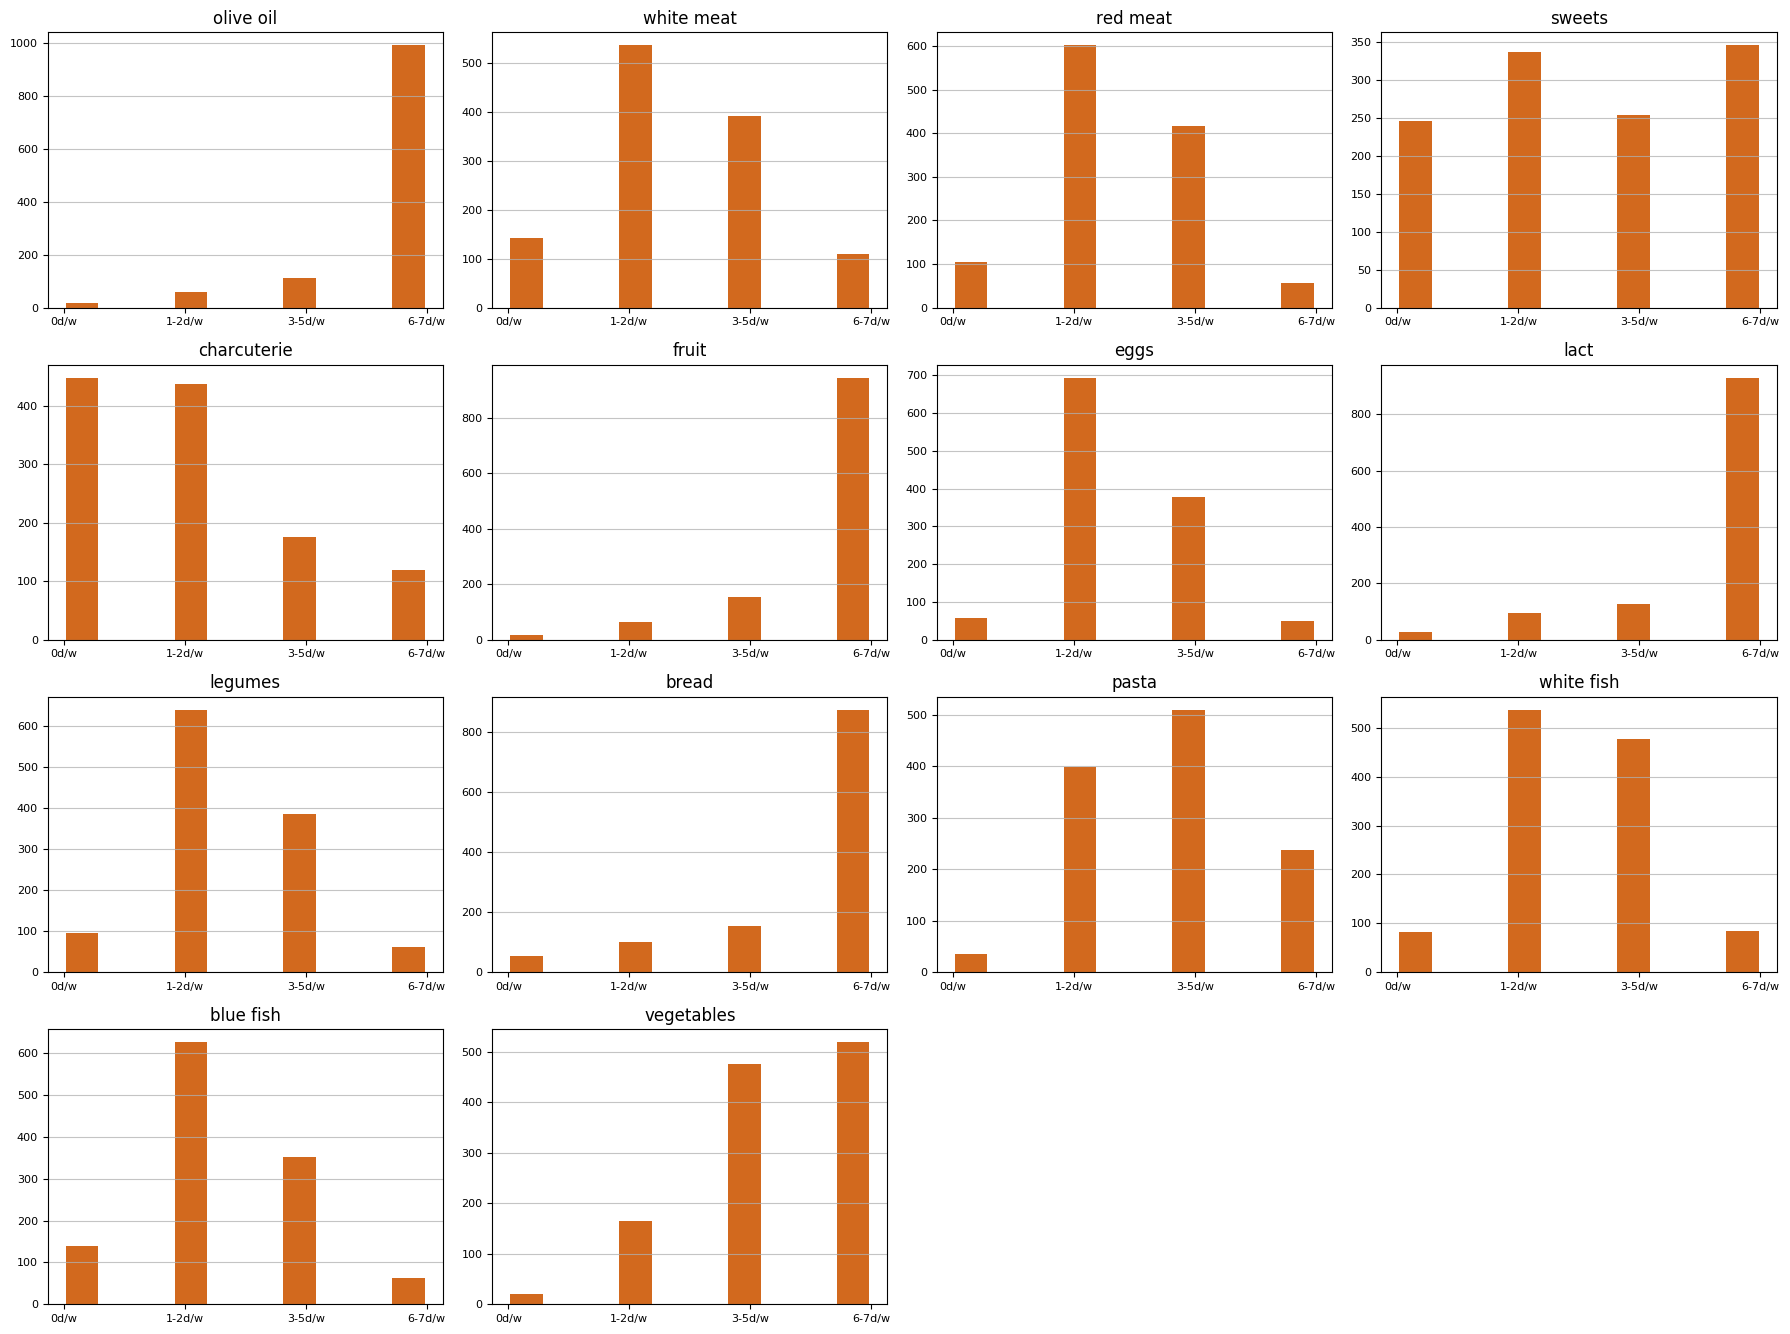
\includegraphics[keepaspectratio, width=\linewidth]{figures/Fig_food}
        \caption{Histogram of type of weekly food consumption reported by the subjects in the first visit. The x-axis of each chart represents how many days a week they consume which type of food. The large majority of subjects report a daily consumption of bread, milk and olive oil. } 
        \label{fig:food}
\end{figure}

%Diet
Figure \ref{fig:diet} depicts the type diet estimated based on the eported weekly food consumption. We distinguish bettwen diet with strong glucemic component (sweets), proteic (cred meat), proteic (eggs, sish meat) and Mediterranean (fruit, fish, vegetables) and we calculate an score for each diet based on REF-MA.

\begin{figure}[H]
        \centering
        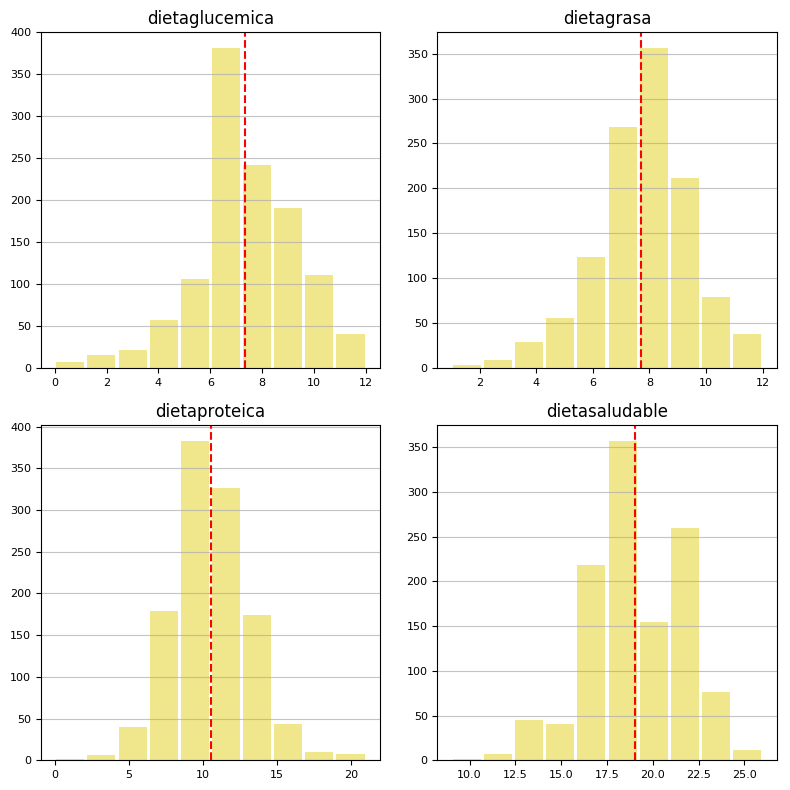
\includegraphics[keepaspectratio, width=0.5\linewidth]{figures/Fig_diet}
        \caption{Histogram of type of diet based on weekly food consumption as reported by the subjects in the first visit. The x-axis of each chart represents the score for each type of diet, the larger the score the most prevalent the main component of the diet is in the subject's diet. For example a subject with a score of 12 in the glucemic diet will likely consume more sweets than a subject a score of 6, by the same token a subject with a large score in the Mediterranean diet will likely consume more fruit and vegetables than a subject with a lower score.} 
        \label{fig:food}
\end{figure}

% Cardiovascular_s ['hta', 'hta_ini', 'glu', 'lipid', 'tabac', 'tabac_cant', 'tabac_fin', 'tabac_ini', 'sp', 'cor', 'cor_ini', 'arri', 'arri_ini', 'card', 'card_ini', 'tir', 'ictus', 'ictus_num', 'ictus_ini', 'ictus_secu']
Figure \ref{fig:cardio} depicts features related to the in the population. The subjects were asked whether they suffer hypertension, angina and heart attack, glucose metabolism disorders, dyslipidemia (an abnormal amount of lipids in the blood), arrhythmias, and if they smoke. 
Thyroid hormones have a significant impact on cardiac function and structure (excess thyroid hormone affects cardiovascular \cite{klein2007thyroid}) and subjects reported whether they suffer from hyper(hipo)thyroidism.
Stroke is a risk factor for coronary heart disease and subjects reported if they had in the past  Hemorrhagic or ischemic cerebral ictus. Ischemic stroke and AD share pathophysiological mechanisms such as inflammation, immune exhaustion and neurovascular damage \cite{lucke2015common}. 
The causality between AD and hemorrhagic stroke seems to be reversed, patients who had Alzheimer's disease are at the highest risk of hemorrhagic stroke \cite{wang2014newly}.
% Pass on sp (you think you are overweighted?) and use If your BMI is 25.0 to <30, it falls within the overweight range. If your BMI is 30.0 or higher, it falls within the obese range

Obesity (Higher midlife BMI) is related to higher risk of dementia and AD, independently of obesity-related risk factors and co-morbidities \cite{tolppanen2014midlife}, \cite{nepal2014rising}. 

The distribution of the BMI of our population is particularly interesting $(BMI_{\mu}=27.3, BMI_{\sigma}=3.6)$. The $26.8\%$ have healthy weight ($BMI \in [18.5, 25]$), $51.8\%$ have over weight ($BMI \in [25,30]$) and $21.4\%$ are obese ($BMI > 30$) \cite{lacruz2015prevalence}. 
The majority of subjects report to have hypertension $53\%$ vs $47\%$, this in line with larger studies 28,887 participants in Spain aged 35-74, high blood pressure was present in $47\%$ in men and $39\%$ in women) \cite{grau2011cardiovascular}.
The $27\%$ are smokers with $33\%$ of ex-smokers.

 %total cholesterol ≥ 250 mg/dL (43% and 40%, respectively), 
 %obesity (29% and 29%, respectively), tobacco use (33% and 21%, respectively), and diabetes (16% and 11%, respectively). Total cholesterol ≥ 190 and ≥ 250 mg/dL were the respective minimum and maximum coefficients of variation (7%-24% in men, 7%-26% in women). Average concordance in lipid measurements between laboratories was excellent. 
%of note the self reported hypertension is inferior to population studies in which the blood pressure is actually measured mean systolic $\geq140$ mmHg and/or diastolic BP (DBP) $\geq90$ mmHg and/or use of antihypertensive medication \cite{lacruz2015prevalence}. 

%https://www.brightfocus.org/alzheimers/article/weight-risk-factor-alzheimers-disease

%https://www.isglobal.org/en/new/-/asset_publisher/JZ9fGljXnWpI/content/cardiopatia-isquemica-demencias-e-ictus-se-situan-como-las-principales-causas-de-muerte-en-espana
\begin{figure}[H]
        \centering
        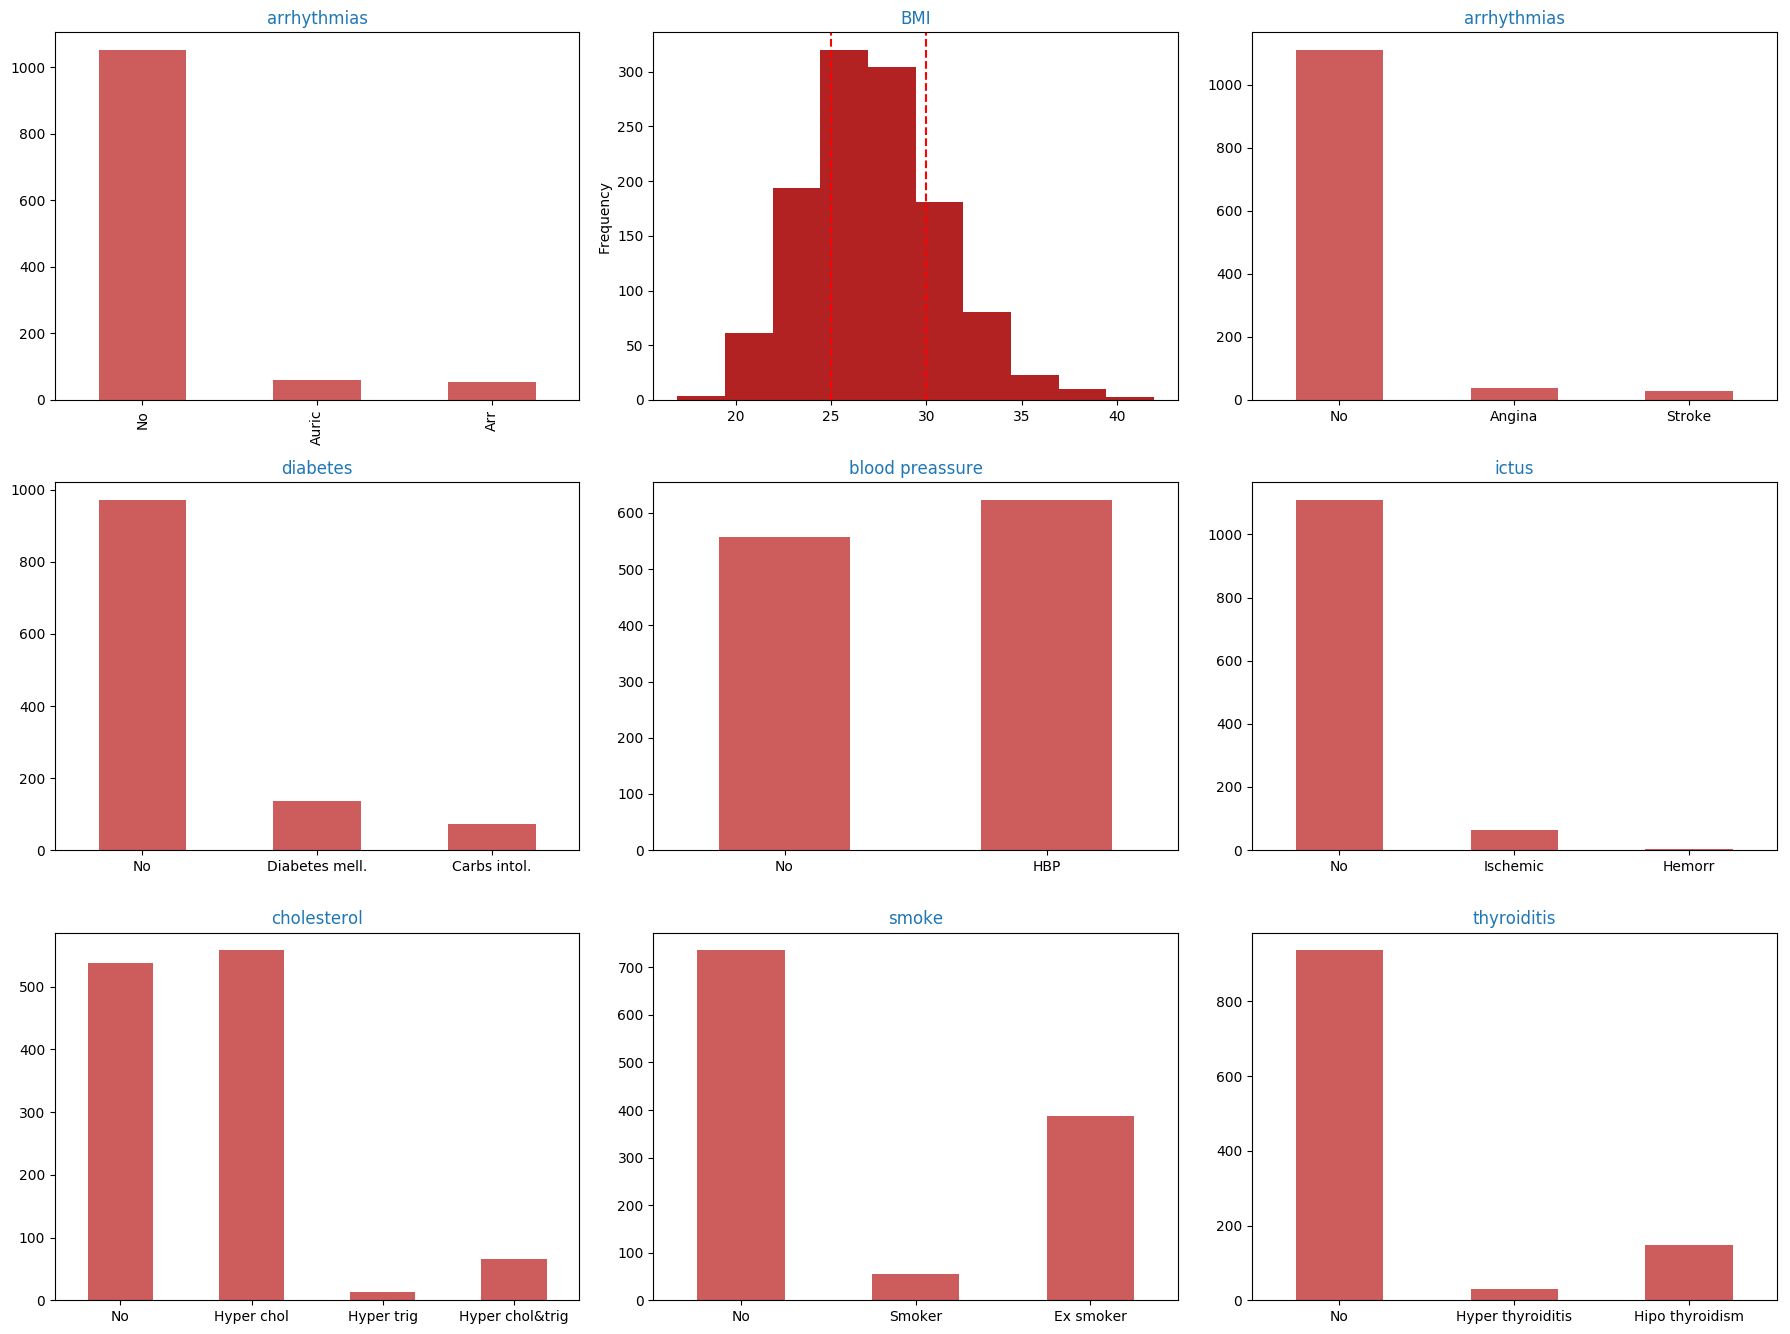
\includegraphics[keepaspectratio, width=0.5\linewidth]{figures/Fig_cardio}
        \caption{Histogram of features related to cardiovascular health. From top down and left to right: arrythmias (No, Atrial fibrillation, Arrhythmia), body mass index, heart stroke (No past strokes, Angina, Stroke), diabetes (No, diabetes mellitus, intollerance to carbs), hypertension, ictus historial (No, Ischemic, Hemorrhagic, cholesterol (No, hyper cholesterol, Hyper triglycerides, both hyper cholesterol and triglycerides), Smoke (No, Smoker, Ex-smoker), thyroiditis (No, Hyper, hipo)) } 
        \label{fig:cardio}
\end{figure}

%PhysicalExercise_s ['ejfre', 'ejminut']
Figure \ref{fig:phys} depicts features related to physical exercise. The subjects were asked the frequency in days per week of the physical exercise and the duration of the sessions.
\begin{figure}[H]
        \centering
        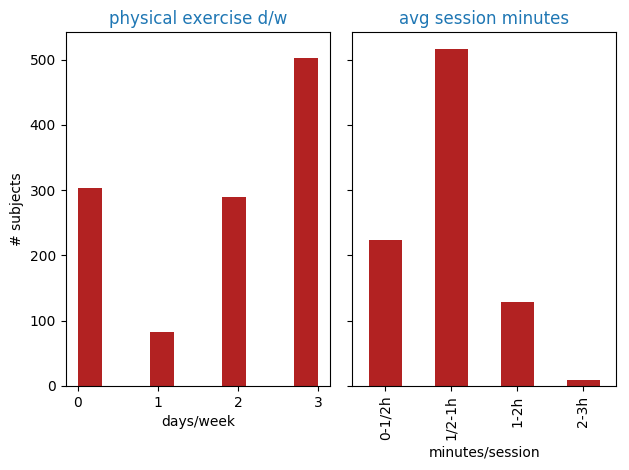
\includegraphics[keepaspectratio, width=0.5\linewidth]{figures/Fig_phys}
        \caption{Histogram of features related to cardiovascular health. From top down and left to right:  } 
        \label{fig:cardio}
\end{figure}

%TraumaticBrainInjury_s ['tce', 'tce_con', 'tce_ini', 'tce_num', 'tce_secu']
%PhysicalExercise_s ['ejfre', 'ejminut']
Figure \ref{fig:tce} shows the distribution of episodes (at least one) of traumatic brain injury. 
\begin{figure}[H]
        \centering
        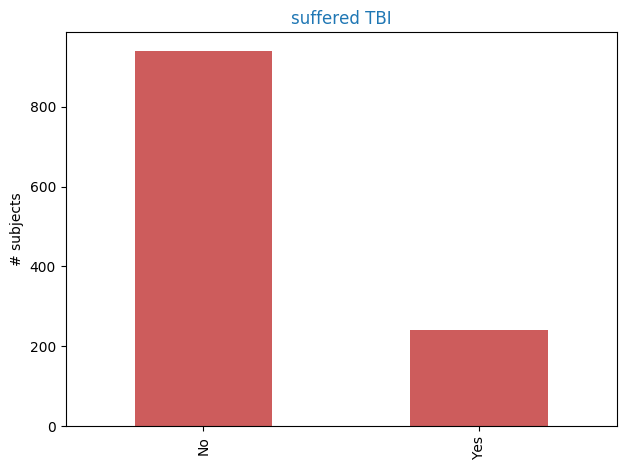
\includegraphics[keepaspectratio, width=0.5\linewidth]{figures/Fig_tce}
        \caption{Histogram of traumatic brain injury. $20\%$ declared to have suffered in the past an episode of  traumatic brain injury of unspecified seriousness.} 
        \label{fig:tce}
\end{figure}

%EngagementExternalWorld_s ['a01', 'a02', 'a03', 'a04', 'a05', 'a06', 'a07', 'a08', 'a09', 'a10', 'a11', 'a12', 'a13', 'a14']

Figure \ref{fig:engage} depicts features related to engagement with the external world of the subject. In particular, do creative activities,  
going out with friends, travel and tourism, community activities (e.g. cultural associations and NGO), going to church, visit social club, go to the movie theater or art shows, go to sport events, how often listens to music, how often watches/listens TVradio , how often reads (books, newspaper, magazines), how often uses the internet.
%EngagementExternalWorld_s ['a03' amigos, 'a04' travel, 'a05' ong, 'a06' church, 'a08' cine, 'a09' sport, 'a10' music, 'a11' tv, 'a12' read, 'a13' internet] 
Church goes are a minority in this sample, $75\%$ never go to church versus $17\%$ that go a few times and $8\%$ that go often. $86\%$ habitually watches the TV or listens to the radio, $68\%$ read books or magazines often and only $29\%$ use the Internet often.

\begin{figure}[H]
        \centering
        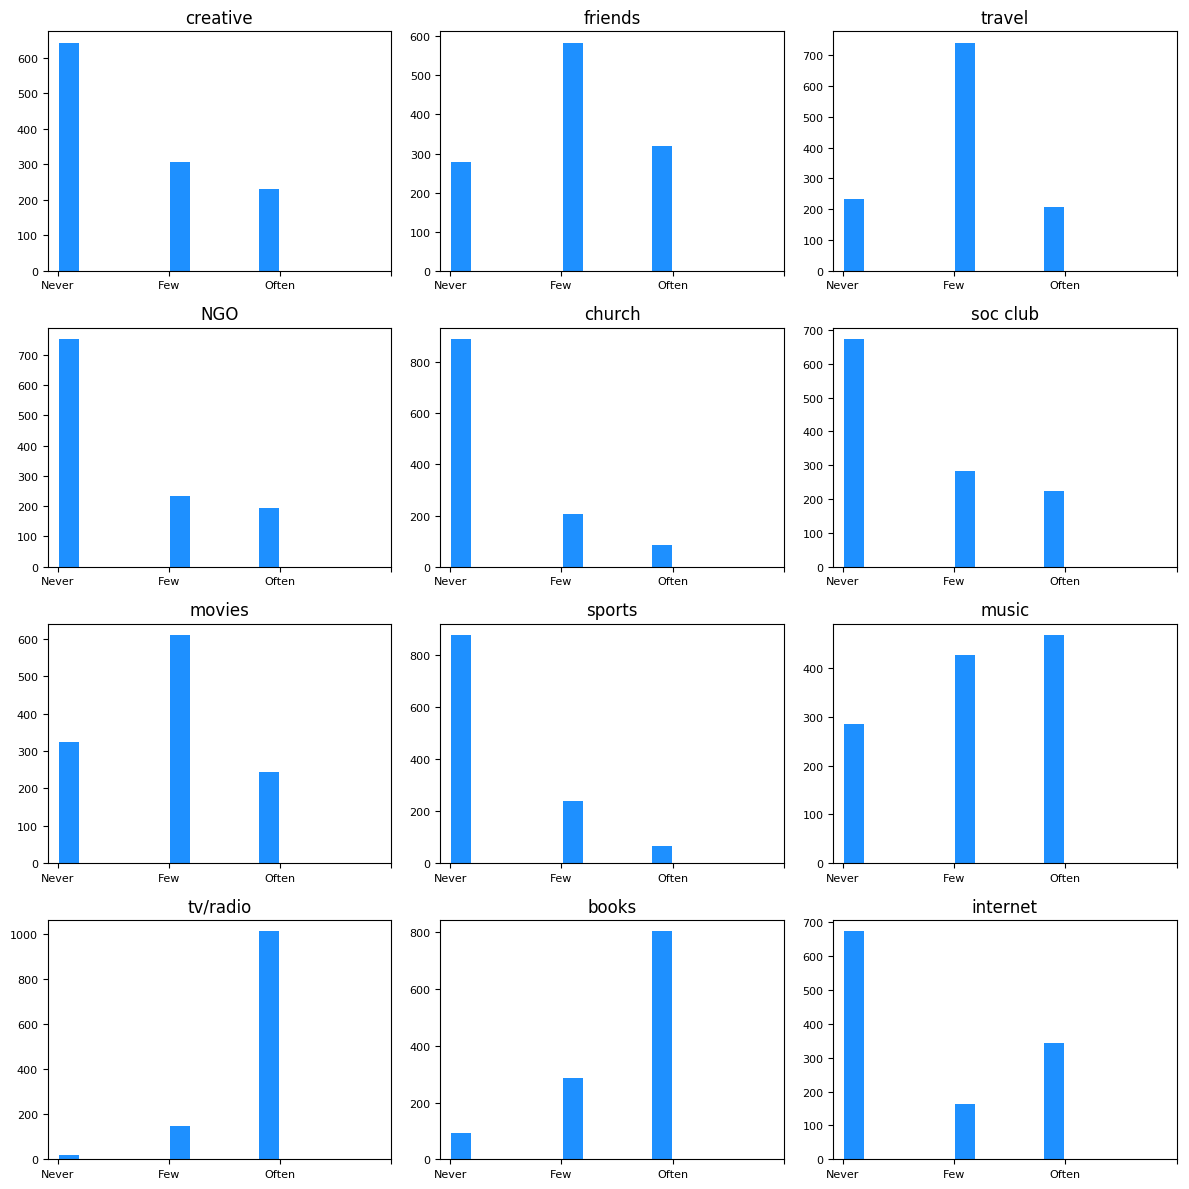
\includegraphics[keepaspectratio, width=0.5\linewidth]{figures/Fig_engage}
        \caption{Histogram of features that reflect engagement with the external world from the part of the subject. From top down and left the charts depict the number of subjects that get involve Never, Few and Often in: creative activities, going out with friends, travel and tourism, community activities (e.g. cultural associations and NGO), going to church, visit social club, go to the movie theater or art shows, go to sport events, how often listens to music, how often watches/listens TVradio , how often reads (books, newspaper, magazines), how often uses the internet.} 
        \label{fig:engage}
\end{figure}

\subsection{Exploratory Data Analysis longitudinal variables}

\section{Methodology}
\label{se:met}
Buschke memory test with free and cued recall is commonly used to assessing persons across levels of cognitive functioning \cite{buschke1973selective}. The Buchske test is of easy realization and can be performed by participants with different levels of impairement and clinical conditions \cite{o200212}, \cite{leitner2017comparison}. The test as was originally conceived designed to asses long-term storage (LTS), retrieval from long-term storage (LTR), and recall from short-term storage (STR).

The test in \emph{Proyecto Vallecas} is divided into two parts, in the first -free recall- the subject is asked to recall words from a list of 16 items. The subject is first give a list of 16 words, and is immediately asked to recall as many the words as possible. Next the subject is distracted with an interference test to be asked again to recall the original 16 words, the subject is distracted again with another interference test to be asked for the third time to recall the original 16 words.

The score consists in three numbers each computes the number of words that the subject correctly recalled at each time. In order to asses retrieval from short/long?-term storage both the total number of items and the increase/decrease in the scores need to be considered. Two subjects with identical aggregate score could have very different recalling. For example, subject A recalls 12, 14 and 15 words at each time and subject B has a score for the same test of 15, 14 and 12. Although both subjects have remember the same number of items, while subject B shows no memory retention (decrease in the number of recalled items) and subject A does consolidate her memory (decrease in the number of recalled items).

We have defined a model that brings together the aggregate of recalled items and the sign of the curve. From calculus we know that the area under a curve between two points can be found by doing a definite integral between the two points. 
The call the three scores in the Buchske  defined in the space of the positive integers, $x \in +\mathbb{Z}^3$, the area under the curve $y = f(x)$ between two points $x=a$ and $x=b$ is the integral between the limits of a and b$\int_{x=a}^{x=b}f(x)dx$ which gives us the area defined by the region $f(x)$ and the boundaries a and b.
Coming back to our original problem we need to calculate not only the area between the interval (a,b) corresponding to the first and the last recall but also the area defined between the first and the second point $(a,h)$ and between the second and the third point $(h,b)$.  
Thus, the quantity S we want to compute is as defined as :
\begin{equation}
S = \int_{a}^{b}f(x)dx + \int_{a}^{h}(f(x) - f(a))dx + \int_{h}^{b}(f(x)-f(h))dx
\label{eq:buchske}
\end{equation}
where the first term on the right side is the area under the curve which gives us an aggregate of the number of items recall, the second and third terms are also areas but contrary to the first term which is always positive $y =f(x)$ is defined only in the positive axis, $y \in [0,16]$ can be negative if the $f(x)$ is decreasing, positive if f(x) is increasing or zero.

Let us see this with an example, for the sake of the argument we assume that the scores are $[0,1,2]$ rather than $[0,1,....16]$. Figure \ref{fig:b} shows the value of S in three different examples. In each case the area is identical, 2, for a total maximum of 4 ($2\times2$ square) but S varies with the learning curve. On the left figure \ref{fig:b}-a,
S is equal to the surface cover because the learning curve is flat, $S=2$. On the middle figure, \ref{fig:b}-b, the scores $S$ is larger than the surface because the curve is increasing (positive slope), $S=2+1/2+1/2=3$. Finally, the figure on the left side, \ref{fig:b}-c, $S=2-1/2-1/2=1$ capturing that the slope is negative and therefore the subject is not consolidating memory.      
  
%https://matplotlib.org/gallery/showcase/integral.html#sphx-glr-gallery-showcase-integral-py
\begin{figure}[H]
        \centering
        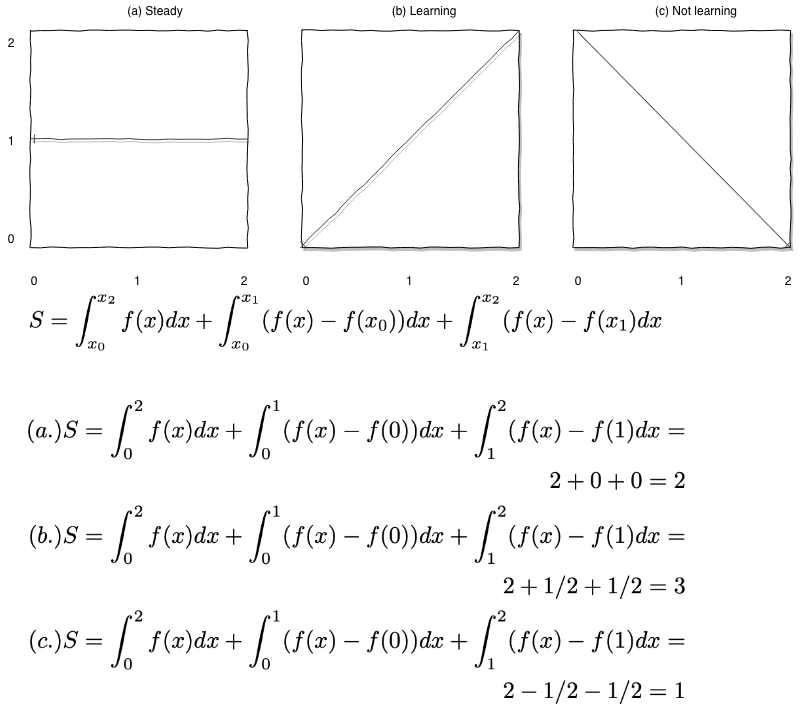
\includegraphics[keepaspectratio, width=\linewidth]{figures/fig_buschkewitheqs}
        \caption{The figure shows the computation of the Buschke scores in three scenarios. On the left figure (a) there is no learning because the subject recalls the same number of items each time ($f(x)=1, x=[0,1,2], S=2$), on the middle figure (b) the subjects learns ($f(x)=x, x=[0,1,2], S=3$) and on the right figure (c) the subject forgets items ($f(x)=-x, x=[0,1,2], S=1$). The maximum score is $S=4$ that would correspond with the subject recalling all the two items at each time ($f(x)=2, x=[0,1,2], S=4$) not shown.} 
        \label{fig:b}
\end{figure}


\section{Results}
\label{se:res}

%tsfresh, Buschke
\section{Conclusions}
\label{se:con}

%-------------------------------------------------------------------------------
% REFERENCES
%-------------------------------------------------------------------------------
\newpage

\addcontentsline{toc}{section}{References}


% BibTeX users please use
\bibliographystyle{spmpsci}
\bibliography{../bibliography-jgr/bibliojgr}

\end{document}